\chapter{Counterfactual Execution Engines}\label{chapter-16-counterfactual-execution-engines}

\begin{quote}
\itshape
Machines that compute by invading and exploring alternative universes.
\end{quote}

This is the chapter where we stop merely observing universes and start invading them.
We are building the machine that moves sideways through possibility \textbf{on purpose}.

Grab the rail. Lean into the pit. We are about to traverse the multiverse.

\definecolor{gridgray}{RGB}{50,50,50}
\definecolor{electricblue}{RGB}{0,200,255}
\definecolor{neonpurple}{RGB}{180,0,255}

\begin{center}
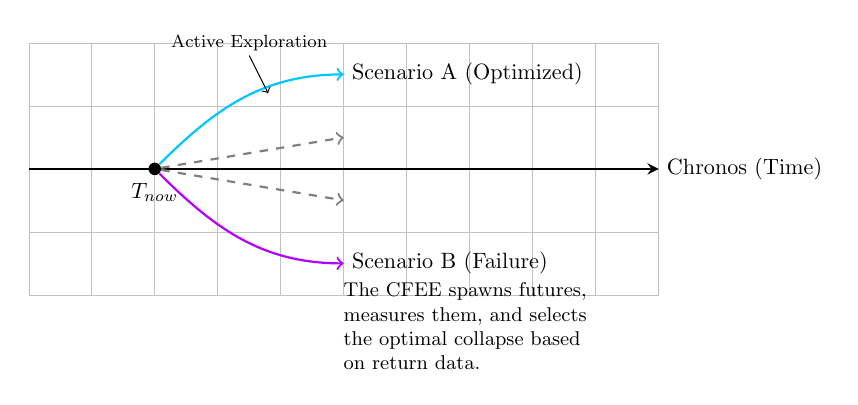
\begin{tikzpicture}[scale=0.8, transform shape]
    % Background Grid
    \draw[step=1cm, gridgray, very thin, opacity=0.3] (-1,-2) grid (9,2);

    % Main Timeline (Chronos)
    \draw[thick, ->, >=stealth] (-1,0) -- (9,0) node[right] {Chronos (Time)};
    
    % Current State
    \node[circle, fill=black, inner sep=2pt, label=below:$T_{now}$] (current) at (1,0) {};

    % Counterfactual Branches (Kairos)
    \draw[thick, electricblue, ->] (current) to[out=45, in=180] (4,1.5) node[right, black] {Scenario A (Optimized)};
    \draw[thick, neonpurple, ->] (current) to[out=-45, in=180] (4,-1.5) node[right, black] {Scenario B (Failure)};
    \draw[thick, gray, dashed, ->] (current) -- (4,0.5);
    \draw[thick, gray, dashed, ->] (current) -- (4,-0.5);

    % The "Probe" Concept
    \node[align=center, font=\footnotesize] at (2.5, 2) {Active Exploration};
    \draw[->, thin] (2.5, 1.8) -- (2.8, 1.2);

    % Annotation
    \node[text width=4cm, align=left, font=\small] at (6, -2.5) {The CFEE spawns futures, measures them, and selects the optimal collapse based on return data.};
\end{tikzpicture}
\end{center}

In Chapter 15, we introduced Time Travel Debugging. That framework allowed us to rewind Chronos, inspect the choices of Kairos, and manually steer the system down different paths. It was a revelation, but it was fundamentally \textit{reactive}. You were the detective arriving at the scene of the crime, rewinding the tape to see who shot the sheriff.

In this chapter, we go further. We stop being detectives and start being navigators.

We are building machines whose entire purpose is to \textbf{actively explore} counterfactual universes as part of their normal operation. These are Counterfactual Execution Engines (CFEEs)—systems that treat alternative futures not as theoretical abstractions, but as first-class computational objects. This marks the transition from single-threaded reality to:

\begin{itemize}
    \item Multiverse search,
    \item Multi-world optimization,
    \item Legal parallel futures,
    \item and Hypothetical execution.
\end{itemize}

You are not simulating possibilities in the colloquial sense of guessing. You are executing actual, legal RMG universes in structured, bounded, computable ways. Let's build the machine.

---

\section{What Is a Counterfactual Execution Engine?}

A Counterfactual Execution Engine is a machine that spawns, evaluates, and selects multiple legal future worldlines from a single root universe.

To understand what it is, we must first clarify what it is not. A CFEE is not a Monte Carlo simulation. It does not guess. It does not approximate. It does not introduce randomness to fuzz the system, nor does it blindly branch into an exponential void.

Instead, a CFEE is a precise geometric operator. It enumerates the ``Bundle''—the finite set of all legal DPO rewrites available at the current tick. It spawns adjacent universes for each valid rewrite, follows those worldlines forward for a bounded duration, and measures the results. It calculates the Rulial Distance to a target state, evaluates the curvature of the local neighborhood, and compares the robustness of competing timelines.

Finally, it collapses back to Chronos. It selects the best path based on concrete data harvested from the futures that didn't happen. This is computation as multiversal navigation.

---

\section{Why Counterfactual Execution Is Safe in RMG+DPO}

In a traditional von Neumann architecture, exploring "what if" scenarios is dangerous and expensive. State is mutable and global; forking a process is heavy; and the space of potential inputs is effectively infinite and unstructured. If you try to explore all reachable states of a standard C++ program, you encounter the halting problem immediately.

But we are in an RMG universe, and that changes the physics of exploration.

\begin{enumerate}
    \item \textbf{Finite Bundles:} At any given tick, the number of valid DPO rule matches is finite.
    \item \textbf{Guaranteed Legality:} Because DPO enforces graph invariants, every spawned universe is guaranteed to be structurally valid. You cannot generate a "corrupt" world, only a different one.
    \item \textbf{Metric Structure:} Rulial Distance gives us a way to measure how "far" a counterfactual is. We aren't searching a void; we are searching a metric space.
    \item \textbf{Deterministic Collapse:} The rules of interference and pruning mean that execution is reproducible.
\end{enumerate}

CFEE does not trigger an exponential explosion because it is constrained by geometry. We explore sideways, but we do so along the defined edges of the Rulial graph.

---

\section{How a Counterfactual Engine Works}

The operational loop of a CFEE is a cycle of expansion and contraction. At each clock tick, the engine performs the following maneuvers:

\textbf{1. Bundle Enumeration} \\
The engine pauses execution and identifies the ``Bundle''—the complete set of legal rewrites that satisfy the current Left-Hand Side (LHS) of the DPO rules.

\textbf{2. Multiverse Spawning} \\
For every valid rewrite in the bundle (or a heuristic subset thereof), the engine spawns a parallel universe. In implementation terms, this is a copy-on-write clone of the RMG state.

\textbf{3. Bounded Forward Exploration} \\
The engine advances each of these parallel universes forward. It applies the standard scheduler to them, respecting all invariants and minimal paths. This exploration is bounded by depth (time ticks) or Rulial Distance (structural change).

\textbf{4. Metric Evaluation} \\
As these worlds evolve, the engine acts as an observer. It computes metrics for each timeline: 
\begin{itemize}
    \item \textit{Distance:} How close is this world to the desired goal state?
    \item \textit{Curvature:} Is this world entering a region of high conflict or deadlock?
    \item \textit{Robustness:} Does this worldline survive small perturbations?
\end{itemize}

\textbf{5. Strategic Collapse} \\
The engine gathers the data and collapses the wave function. It selects the worldline that optimizes the desired metric—be it safety, speed, or stability—and discards the others. The system then proceeds along that optimal path in the "real" timeline (Chronos).

This is not "branch and bound" in the traditional sense. This is navigating a structured manifold of possibilities.

\begin{center}
\begin{tikzpicture}[node distance=2cm]
    % Nodes
    \node (start) [rectangle, draw, rounded corners, fill=white, text width=3cm, align=center] {Current RMG State};
    \node (bundle) [trapezium, draw, trapezium left angle=70, trapezium right angle=110, fill=gray!10, below of=start, text width=2.5cm, align=center] {Compute Bundle};
    
    \node (world1) [circle, draw, fill=electricblue!20, below left of=bundle, xshift=-1cm] {$W_1$};
    \node (world2) [circle, draw, fill=electricblue!20, below of=bundle] {$W_2$};
    \node (world3) [circle, draw, fill=electricblue!20, below right of=bundle, xshift=1cm] {$W_3$};
    
    \node (eval) [rectangle, draw, fill=white, below of=world2, text width=4cm, align=center] {Evaluate Metrics (Distance, Curvature)};
    
    \node (collapse) [rectangle, draw, rounded corners, fill=black, text=white, below of=eval] {Collapse to Optimal};

    % Arrows
    \draw[->, thick] (start) -- (bundle);
    \draw[->, thick] (bundle) -- (world1);
    \draw[->, thick] (bundle) -- (world2);
    \draw[->, thick] (bundle) -- (world3);
    \draw[->, dashed] (world1) -- (eval);
    \draw[->, dashed] (world2) -- (eval);
    \draw[->, dashed] (world3) -- (eval);
    \draw[->, thick] (eval) -- (collapse);
    
    % Labels
    \node[right of=bundle, xshift=2cm, align=left, text width=3cm, font=\footnotesize] {Identify all legal DPO matches};
    \node[right of=world3, xshift=1cm, align=left, text width=3cm, font=\footnotesize] {Bounded Execution};
\end{tikzpicture}
\end{center}

---

\section{Counterfactual Execution in Practice}

How do we actually use this engine? It transforms abstract problems into geometric searches.

\subsection{Search and Optimization}
In a traditional system, finding an optimal state often requires gradient descent or heuristic guessing. In a CFEE, optimization is a pathfinding problem. The engine can look ahead into multiple futures, evaluating the "cost" of each path, and selecting the rewrite that lowers the Rulial Distance to the goal.

\subsection{Reasoning and Hypothesis Testing}
This is the most powerful application. The engine can ask, ``What happens if I apply Rule A instead of Rule B?'' It doesn't need to guess; it runs the simulation. It allows the system to test hypotheses: ``If I open this wormhole, will it violate a security invariant 10 ticks from now?'' The engine explores that future, detects the violation, and prunes that choice in the present.

\subsection{Fault Tolerance and Model Selection}
The CFEE can act as a resilience engine. Before committing to a transaction, it can simulate a failure in that transaction's dependencies. If the simulated future leads to a catastrophic unrecoverable state, the engine can proactively choose a different, more robust path. It explores the ``Model Rule'' axis to find the universe most resistant to error.

---

\section{The Time Cube as Input}

We previously discussed the Time Cube (Chapter 5) as a theoretical construct—a visualization of local history and future possibility. For the CFEE, the Time Cube is not a diagram; it is the input data structure.

The ``Bundle'' is the entry point. The ``Light Cone'' is the horizon of the search depth. The ``Neighborhoods'' define the structure of the search space. When the CFEE runs, it is literally reading the geometry of the Time Cube to make decisions. This is what makes RMG+DPO a computational substrate rather than just a model: the geometry *is* the logic.

---

\section{Counterfactual Engines Respect Determinism}

There is a common misconception that exploring multiple possibilities implies non-determinism or randomness. This is false.

\textbf{Counterfactuality does not introduce non-determinism.}

Each parallel universe spawned by the CFEE is internally consistent and fully deterministic. It has one collapse history, one scheduler, and one valid worldline. When the CFEE explores ten different futures, it is engaging in \textbf{Parallel Determinism}. 

We are not rolling dice. We are essentially running ten different, perfectly rigorous clocks side-by-side. This makes the system safe, verifiable, and totally computable.

---

\section{Avoiding Branch Explosion}

The specter of exponential explosion haunts any discussion of branching paths. Why doesn't the CFEE crash the system by spawning billions of universes?

The answer lies in the structure of RMGs. The search space is heavily constrained by:
\begin{itemize}
    \item \textbf{Interference:} Many rules are mutually exclusive. Picking one prunes the others immediately.
    \item \textbf{Invariants:} Any path that violates a graph invariant is instantly terminated.
    \item \textbf{Geodesics:} We are usually interested in the "shortest path" or the "minimal collapse." This focus allows us to ignore the vast majority of convoluted, high-entropy paths.
    \item \textbf{Structure Sharing:} Because these are graph rewrites, large portions of the state graph remain identical across universes. We can structurally share memory, meaning ten universes don't cost ten times the RAM.
\end{itemize}

The result is an exploration profile that feels exponential in power but behaves polynomially in resource consumption.

---

\section{Counterfactual Execution as a Reasoning Engine}

We reach the hype peak of the chapter. A Counterfactual Execution Engine is, effectively, a reasoning machine.

Consider how humans reason. When you decide to cross the street, you quickly simulate: ``If I step out now, the bus hits me. If I wait, the bus passes.'' You explore two counterfactual worldlines, evaluate the termination state (Death vs. Survival), and collapse your reality to the choice that leads to Survival.

The CFEE gives \COMPUTER{} this exact capability. It allows the system to:
\begin{itemize}
    \item Test hypotheses ("If I do X..."),
    \item Simulate alternate histories ("...then Y happens."),
    \item And choose optimal worldlines ("Therefore, I will wait.").
\end{itemize}

You have just given computation its first real meta-cognitive engine. It is not AI in the neural network sense. It is not consciousness. It is \textbf{Structured Counterfactuality}.

\begin{nerdbox}
\textbf{CFEE = Multiverse Search Over Rulial Neighborhood Graphs}

Formally, a CFEE is performing a traversal of the local Rulial Neighborhood Graph.
\begin{itemize}
    \item The **Time Cube** represents the local branching factor of the graph.
    \item **Interference** is effectively a joinability analysis or Critical Pair analysis.
    \item **Collapse** corresponds to a specific reduction sequence in the rewrite system.
\end{itemize}
In term rewriting systems, we often discuss "Confluence"—the idea that different rewrite paths eventually converge. CFEE is an operationalized confluence analyzer. It explores the Critical Pairs to find the normalization path that minimizes a specific cost function defined by Rulial Distance.
\end{nerdbox}

---

\section{Transition: From Counterfactual Engines to Adversarial Universes}

We have built Time Travel Debugging (Chapter 15) to fix the past.
We have built Multiverse Execution (Chapter 16) to optimize the future.

But what if the multiverse hates you?

Now we must build adversaries—intelligent agents that live across these universes, specifically designing inputs and rule sequences to break your invariants. These are the \textbf{MORIARTY} engines.

\textbf{Next: Chapter 17 --- Adversarial Universes (MORIARTY)}
